\documentclass{article}

\usepackage[preprint]{neurips}
\usepackage[utf8]{inputenc}
\usepackage[T1]{fontenc}
\usepackage{amsmath,amssymb,amsfonts}
\usepackage{booktabs}
\usepackage{graphicx}
\usepackage{microtype}
\usepackage{xcolor}
\usepackage{url}
\usepackage{hyperref}

\title{Understanding Attention: A Worked Guide to Transformer Reasoning}
\author{Lattice Tutorial \\
An editable, collaborative example project \\
\texttt{hello@lattice.example}}

\begin{document}
\maketitle

\begin{abstract}
Attention turns a collection of token representations into context-sensitive representations by learning which pieces of information should interact.
This tutorial develops that operation from a small numerical example, connects it to multi-head self-attention and the Transformer block, and surveys several influential extensions.
The manuscript is deliberately written as a compact NeurIPS-style research note so that it can demonstrate editing, citation management, figures, and collaboration inside Lattice.
All diagrams and prose in this project are original teaching material; cited papers remain the sources for architectural and empirical claims.
% Tutorial: revise the final sentence above, then select Build to see the PDF update.
\end{abstract}

\section{From sequence models to attention}

A sequence model must decide how information at one position can influence another.
Recurrent neural networks pass a hidden state from left to right, creating a path whose length grows with token distance.
Additive attention introduced a learned alignment mechanism that let a decoder retrieve different encoder states instead of compressing an entire source sentence into one fixed vector \citep{bahdanau2015neural}.
Multiplicative variants made this retrieval efficient and became a standard component of neural machine translation systems \citep{luong2015effective}.

The Transformer made a stronger design choice: attention became the principal mechanism for communication between positions, while recurrence and convolution disappeared from the main sequence-processing path \citep{vaswani2017attention}.
That choice exposes parallel computation during training and gives every pair of positions a direct interaction path within a layer.
It does not make sequence modeling free: dense attention stores a score for every query--key pair, producing quadratic time and memory growth in sequence length.
Later work therefore explores sparse, kernelized, recurrent, and hardware-aware alternatives \citep{tay2022efficient,choromanski2021rethinking,dao2022flashattention}.

\section{Scaled dot-product attention}

Let $X\in\mathbb{R}^{n\times d}$ contain one representation for each of $n$ tokens.
Learned projections produce queries, keys, and values,
\begin{equation}
  Q=XW_Q,\qquad K=XW_K,\qquad V=XW_V.
\end{equation}
The output is
\begin{equation}
  \operatorname{Attention}(Q,K,V)
  = \operatorname{softmax}\!\left(\frac{QK^\top}{\sqrt{d_k}}\right)V.
  \label{eq:attention}
\end{equation}
Each row of $QK^\top$ contains compatibility scores between one query and all keys.
The row-wise softmax converts those scores into non-negative weights that sum to one, and the weighted sum of value vectors forms the output for that query.
The factor $1/\sqrt{d_k}$ controls score magnitude: if query and key coordinates have roughly unit variance, their dot product variance grows with $d_k$, which can push softmax into regions with very small gradients \citep{vaswani2017attention}.

\subsection{A numerical example}

Consider the four-token fragment ``attention connects every position.''
For the query at \emph{connects}, suppose the scaled scores are $[0.4,1.2,0.1,0.8]$.
Applying softmax gives approximately $[0.18,0.41,0.14,0.27]$ after rounding.
The new representation at \emph{connects} is therefore a convex combination of all four value vectors, with the largest contribution coming from its own value in this illustrative head.
Changing the softmax temperature alters concentration but not the underlying value vectors; the interactive HTML file in this project lets the reader inspect that distinction.

\begin{figure}[t]
  \centering
  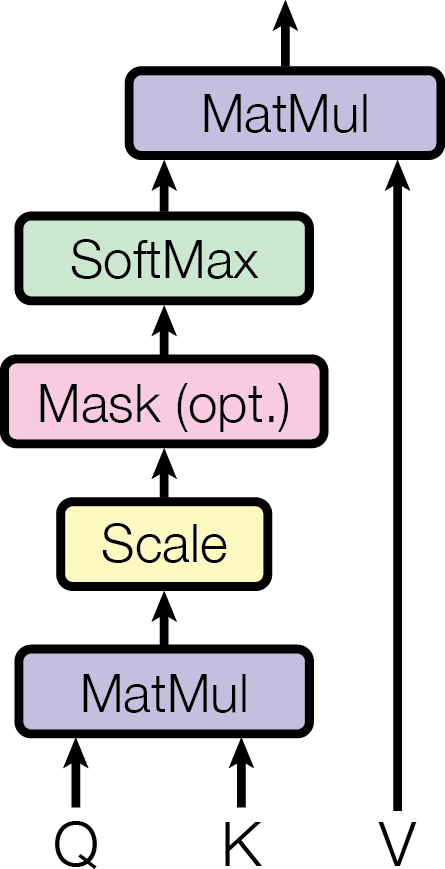
\includegraphics[height=.25\textheight]{figures/scaled-dot-product-attention.png}
  \hfill
  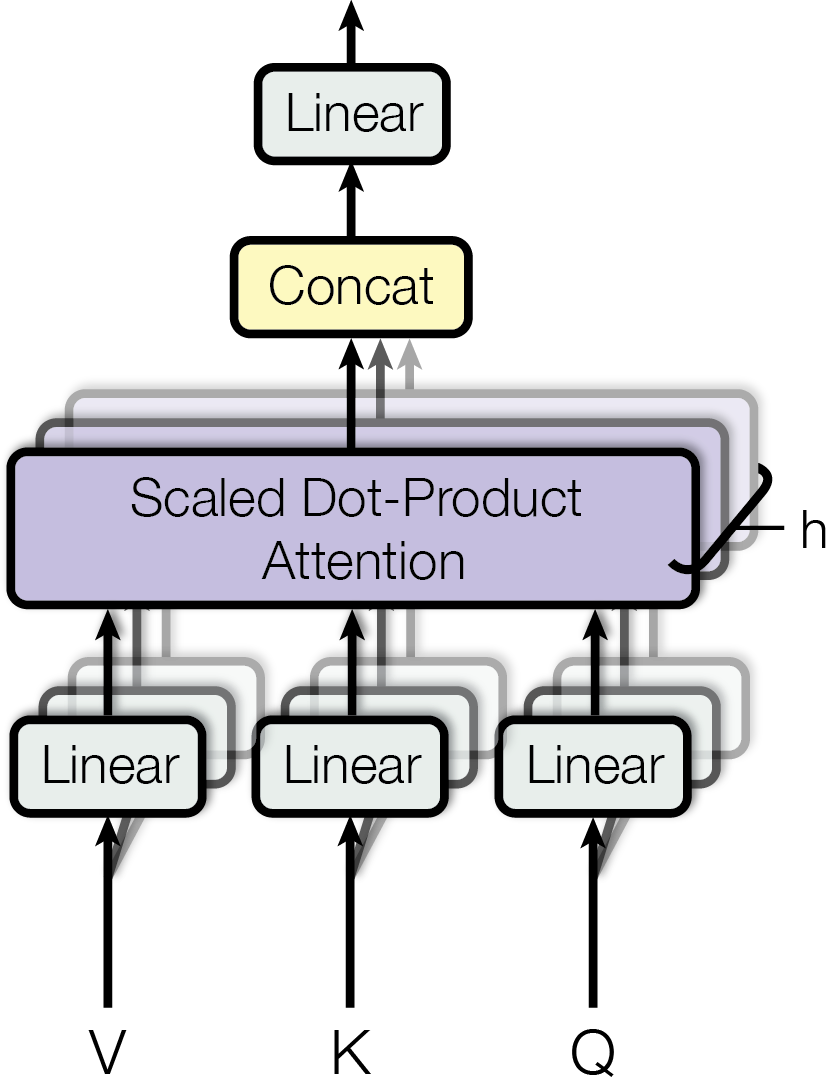
\includegraphics[height=.25\textheight]{figures/multi-head-attention.png}
  \caption{Scaled dot-product attention (left) and multi-head attention (right), reproduced from Figure~2 of \citet{vaswani2017attention} with permission from Google for use in scholarly works.}
  \label{fig:attention-map}
\end{figure}

\section{Multi-head attention and Transformer blocks}

A single attention distribution offers one way to route information.
Multi-head attention applies several sets of projections in parallel,
\begin{align}
  \operatorname{head}_i &= \operatorname{Attention}(QW_i^Q,KW_i^K,VW_i^V),\\
  \operatorname{MHA}(Q,K,V) &= \operatorname{Concat}(\operatorname{head}_1,\ldots,\operatorname{head}_h)W^O.
\end{align}
Different heads are free to learn different interactions, although a head should not automatically be interpreted as a clean linguistic rule.
Attention visualizations describe routing weights inside a model, not a causal explanation of the model's final prediction.

In an encoder block, multi-head self-attention is followed by a position-wise feed-forward network, with residual connections and normalization around sublayers.
Because self-attention alone is permutation equivariant, the model also receives positional information.
The original Transformer used sinusoidal encodings \citep{vaswani2017attention}; many later architectures use learned or relative position representations.
Masking changes which keys are visible: bidirectional encoders such as BERT can condition on tokens on both sides \citep{devlin2019bert}, whereas autoregressive language models mask future positions so generation remains causal \citep{brown2020language}.

\section{Where the pattern is used}

The same computation supports several application regimes.
BERT scales bidirectional Transformer encoders and adapts them to language understanding through pretraining and fine-tuning \citep{devlin2019bert}.
GPT-3 studies autoregressive scaling and in-context task specification without gradient updates at evaluation time \citep{brown2020language}.
Vision Transformers divide an image into patches and process the resulting sequence with a largely standard Transformer encoder \citep{dosovitskiy2021image}.
These systems differ in objective, masking, data, and scale, so ``uses attention'' is only the beginning of an architectural description.

\begin{table}[t]
  \centering
  \caption{Representative uses of Transformer attention. The table summarizes architectural roles rather than comparing reported scores across incompatible tasks.}
  \label{tab:applications}
  \begin{tabular}{@{}llll@{}}
    \toprule
    System & Input unit & Visibility & Representative use \\
    \midrule
    Transformer & Text token & Encoder / causal & Translation \\
    BERT & WordPiece & Bidirectional & Language understanding \\
    GPT-3 & Text token & Causal & Autoregressive generation \\
    ViT & Image patch & Bidirectional & Image classification \\
    \bottomrule
  \end{tabular}
\end{table}

\section{Efficiency and implementation}

For sequence length $n$, dense attention materializes an $n\times n$ score matrix.
Approximation methods reduce this cost by restricting interactions or rewriting the softmax computation.
The Performer, for example, approximates softmax attention with random features and computes associations without explicitly storing the full attention matrix \citep{choromanski2021rethinking}.
The broader design space includes fixed patterns, learned sparsity, low-rank projections, recurrence, and memory mechanisms; a survey by \citet{tay2022efficient} organizes these approaches and their trade-offs.

Algorithmic complexity is only part of runtime behavior.
FlashAttention computes exact attention while tiling operations to reduce expensive transfers between levels of GPU memory \citep{dao2022flashattention}.
This distinction is useful when evaluating a claimed improvement: an approximation changes the mathematical operation, whereas an input/output-aware kernel can preserve the operation but execute it more efficiently on specific hardware.
Benchmarks should report sequence length, precision, hardware, memory use, and end-to-end context because asymptotic notation alone cannot predict practical speed.

\section{What attention does not establish}

Attention weights can be inspected, but inspection does not by itself identify why a model produced an output.
Weights are conditioned on learned representations, interact with residual streams and feed-forward layers, and may be transformed by later blocks.
Likewise, long-range connectivity does not guarantee reliable long-context reasoning: optimization, positional representation, data coverage, and retrieval behavior still matter.
A careful analysis combines mechanistic probes with controlled interventions and task-level evaluation rather than treating one heat map as a complete explanation.

\section{Reproducible learning workflow}

This repository is also a worked example of a research workspace.
The LaTeX source uses the bundled NeurIPS 2026 preprint style; \texttt{notes.md} separates reading notes from publication prose; \texttt{attention-demo.html} provides an interactive explanation; and \texttt{figures/} contains the cited source panels and a publication-ready PDF copy.
The bibliography gives the Papers panel several records to manage.
Before adding a new factual claim, import or open its source, record the evidence in the notes, make the manuscript change, and review the resulting project history with collaborators.

\section{Conclusion}

Scaled dot-product attention is a compact routing operation: compare queries with keys, normalize the scores, and mix values.
Multi-head projections, positional information, masking, residual computation, data, and implementation strategy turn that operation into a useful model.
Understanding those surrounding choices prevents the attention equation from becoming an explanation that is simultaneously familiar and incomplete.

\bibliographystyle{plainnat}
\bibliography{references}

\end{document}
